\documentclass{amsart}
\usepackage{amsmath,amssymb,amsthm,fullpage,mathptmx, hyperref,dsfont,framed, graphicx, subcaption, textcomp, tikz} % The usual suspects

%%%%%%%%%%%%%%%%%% Tikz %%%%%%%%%
\usepackage{tikz}
\usetikzlibrary{shapes.geometric}
\usetikzlibrary{calc}
\usetikzlibrary{scopes}
\usetikzlibrary{decorations.markings}

\tikzset{
every picture/.style={line width=0.8pt, >=stealth,
                       baseline=-3pt,label distance=-3pt},
%%%%%%%%%%  Node styles
dotnode/.style={fill=black,circle,minimum size=2.5pt, inner sep=1pt, outer
sep=0},
morphism/.style={circle,draw,thin, inner sep=1pt, minimum size=15pt,
                 scale=0.8},
small_morphism/.style={circle,draw,thin,inner sep=1pt,
                       minimum size=10pt, scale=0.8},
coupon/.style={draw,thin, inner sep=1pt, minimum size=18pt,scale=0.8},
%%%% different line styles:
regular/.style={densely dashed},
edge/.style={thick, dashed, draw=blue, text=black},
boundary/.style={thick,  draw=blue, text=black},
overline/.style={preaction={draw,line width=2mm,white,-}},
drinfeld center/.style={>=stealth,green!60!black, double
distance=1pt,text=black},
%%%%%%% Fill styles %%%%%%%%%%%%%%%
cell/.style={fill=black!10},
subgraph/.style={fill=black!30},
%%%%%%% Mid-path arrows
midarrow/.style={postaction={decorate},
                 decoration={
                    markings,% switch on markings
                    mark=at position #1 with {\arrow{>}},
                 }},
midarrow/.default=0.5
}



\newtheorem{thm}{Theorem}[section]
\newtheorem*{uthm}{Theorem}
\newtheorem{lem}[thm]{Lemma}
\newtheorem*{ulem}{Lemma}
\newtheorem{prop}[thm]{Proposition}
%\newtheorem*{uprop}[thm]{Proposition}
\newtheorem{cor}[thm]{Corollary}
\newtheorem{conj}[thm]{Conjecture}
\newtheorem{defn}[thm]{Definition}
\newtheorem{rmk}[thm]{Remark}
\newtheorem{prob}[thm]{Open problem}
\newtheorem{ques}[thm]{Question}
\newtheorem{fact}[thm]{Fact}
\newtheorem{ex}[thm]{Exercise}


\DeclareMathOperator{\MCG}{MCG}
\DeclareMathOperator{\Vect}{Vec}
\DeclareMathOperator{\Homeo}{Homeo}
\DeclareMathOperator{\Hom}{Hom}
\DeclareMathOperator{\Obj}{Obj}
\DeclareMathOperator{\Irr}{Irr}
\DeclareMathOperator{\Img}{Im}

\begin{document}

\title{Finiteness for Mapping Class Group Representations from Twisted Dijkgraaf-Witten Theory}


\author{Paul Gustafson}
\email{pgustafs@math.tamu.edu}
\address{Department of Mathematics,
    Texas A\&M University,
    College Station, TX
    U.S.A.}
    
\maketitle

\begin{figure}
    \centering
    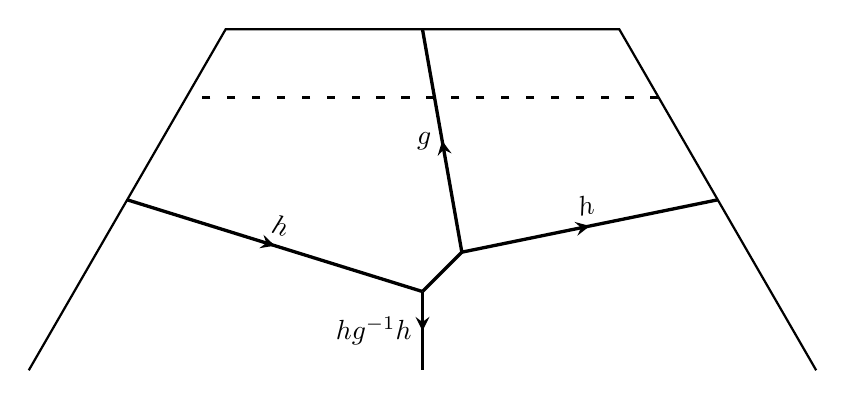
\begin{tikzpicture}[scale=5]
    
    %cut
    \draw[loosely dashed] (0.6, 0.6928) -- (-0.6, 0.6928);
    
    %boundary of polygon
    \path[draw] (1,0) -- (1/2, 0.866) -- (-1/2, 0.866) -- (-1, 0);

    %graph edges
    \begin{scope}[very thick,decoration={
    markings,
    mark=at position 0.5 with {\arrow{>}}}
    ] 
        \draw[postaction={decorate}]  (0.1, 0.3) -- (0.75, 0.433) node[pos=.5,sloped,above]{$h$};
        \draw[postaction={decorate}]  (0.1, 0.3) -- (0, 0.866) node[pos=.5,left]{$g$};
        \draw[postaction={decorate}]  (-0.75, 0.433) -- (0, 0.2) node[pos=.5,sloped,above]{$h$};
        \draw[postaction={decorate}]  (0, 0.2) -- (0, 0) node[pos=.5,left]{$hg^{-1}h$};
        \draw (0, 0.2) -- (0.1, 0.3);
    \end{scope}
    \end{tikzpicture}
    \caption{First type of Dehn twist}
    \label{fig:tikzTwist1_1}
\end{figure}

%TODO write program to output files


\end{document}
